\documentclass[12pt,a4paper]{article}
\usepackage{hyperref}
\usepackage{float}
\usepackage{graphicx}
\usepackage[utf8]{inputenc}
\usepackage{amsmath}
\usepackage{amsfonts}
\usepackage{amssymb}
\author{Howard Cheung \\ email: howard.at (at) gmail.com }
\title{User manual for the Data Preprocessing Helper Version 0.3.3}
\begin{document}

\maketitle

\tableofcontents

\section{Introduction}

This tool is made to assist data analysts who are unfamiliar with coding languages to preprocess their time-series data.
In a lot of engineering systems, data from different subsystems are obtained differently.
While some of them are obtained at different fixed time intervals, some of them, such as on/off signals, are obtained at times when the signal changes.
Some other data contain invalid or missing data points that results in invalid calculation.
Some users may like numerical values over time string characters for their calculation.
The resultant data are very difficult for laymen who only use spreadsheet software to analyze their data.
This project aims at helping these analysts to preprocess their data by converting the time-of-value-change data to data collected at fixed time intervals.

\section{Pre-requisites}
This section discusses the requirements for the computer and the data for the use of the Data Preprocessing Helper.

\subsection{Computer}
The executable of the software is built for computers running 64-bit Windows Operation Systems.
It may be able to operate on other 64-bit Windows computers but is not tested with it.
For users using other operating systems, they can build the executable using the instructions at \href{https://github.com/howardcheung/data-preprocessing-helper/blob/master/exe/README.md}{here}.

\subsection{Data}
The data file should be in the format of either a csv file (comma-separated file), an xls file (Microsoft Excel 1997-2003 file) or an xlsx file (Microsoft Excel Open XML Format file). Their detailed requirements are discussed below.

\subsubsection{csv file}
\label{sec:csv-file}
csv files are files which data are stored with ',' or ';' as delimiters. For data in csv format to work with the Data Preproessing Helper, its data must be structured as follows.

\begin{enumerate}
\item The first column of data must be data with date and time. It can contain date only if the data are acquired at day intervals.
\item The data beyond the first column must be separated by either ',' or ';'.
\item It can contain multiple rows above the data, but only the first row above the data will be considered as the header.
\end{enumerate}

An example of the data file is shown in Figure \ref{fig:csv_file}.

\begin{figure}[H]
\centering
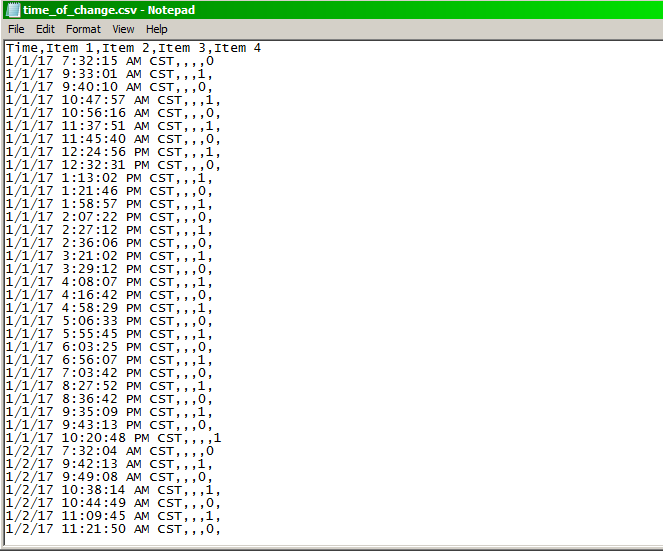
\includegraphics[width=0.8\textwidth]{csv-file.png}
\caption{Example csv file that can be processed by Data Preprocessing Helper}
\label{fig:csv_file}
\end{figure}

\subsection{xls and xlsx files}
xls and xlsx files are used as spreadsheet files, and the requirements for them to be preprocessed by the Data Preprocessing Helper are the same. For each worksheet inside the files, the data must be aligned to follow these requirements:

\begin{enumerate}
\item The first column of data must be data with date and time. It can contain date only if the data are acquired at day intervals.
\item It can contain multiple rows above the data, but only the first row above the data will be considered as the header.
\end{enumerate}

If the user would like to preprocess multiple worksheets in a file simultaneously, the format of data in each worksheet must be the same.
For example, the format of the time string in the first columns in all worksheets in a file must be the same, and the number of rows above the first row of data must be the same as well.
An example is given in Figure \ref{fig:xls_file}.

\begin{figure}[H]
\centering
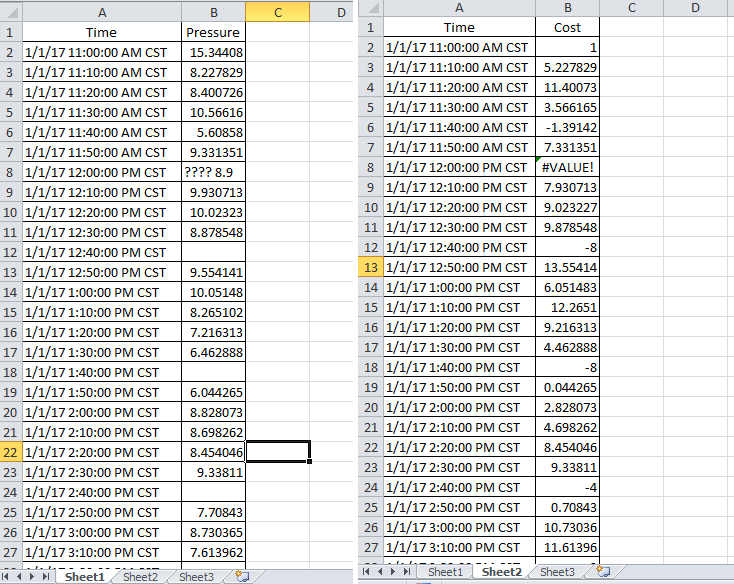
\includegraphics[width=0.8\textwidth]{xls-file.png}
\caption{Example xls file with two worksheets that can be processed by Data Preprocessing Helper}
\label{fig:xls_file}
\end{figure}

\section{Tutorial}

\subsection{Conversion of time-of-value-change data to data at fixed time interval}

This tutorial gives a quick tour on how to convert a file with time-of-value-change data to a file at fixed time intervals.
First we start with a csv file with the structure in Figure \ref{fig:ugly_file}.

\begin{figure}[H]
\centering
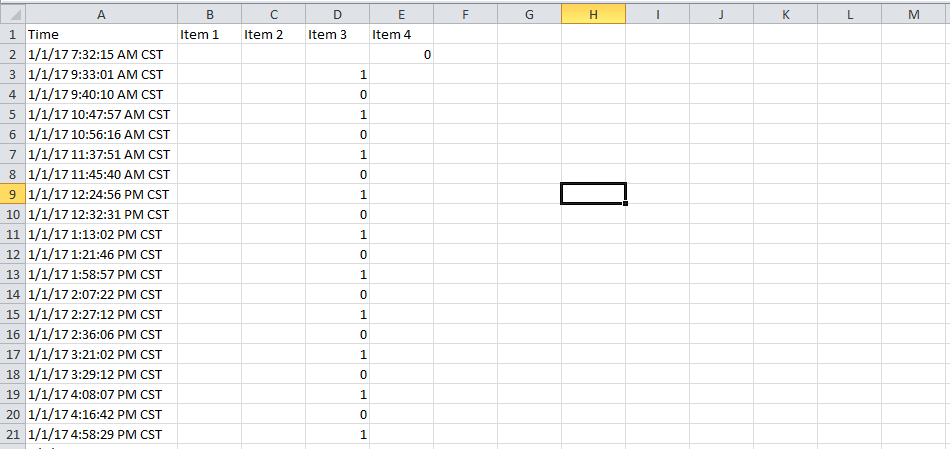
\includegraphics[width=0.8\textwidth]{time-of-change.png}
\caption{Structure of data with time-of-change values}
\label{fig:ugly_file}
\end{figure}

As you can see, there are a lot of unavailable values in Figure \ref{fig:ugly_file}.
The timestamps on the left are also ugly because they are all acquired at different time intervals.
It is very difficult to try comparing this set of data side-by-side with the other data set.

To convert the data in Figure \ref{fig:ugly_file}, we can use the tool provided in this project.
The tool is wrapped as an executable so that you don't have to worry about linking your confidential data to the web to do the filtering.
Its user interface is shown in Figure \ref{fig:ui}.

\begin{figure}[H]
\centering
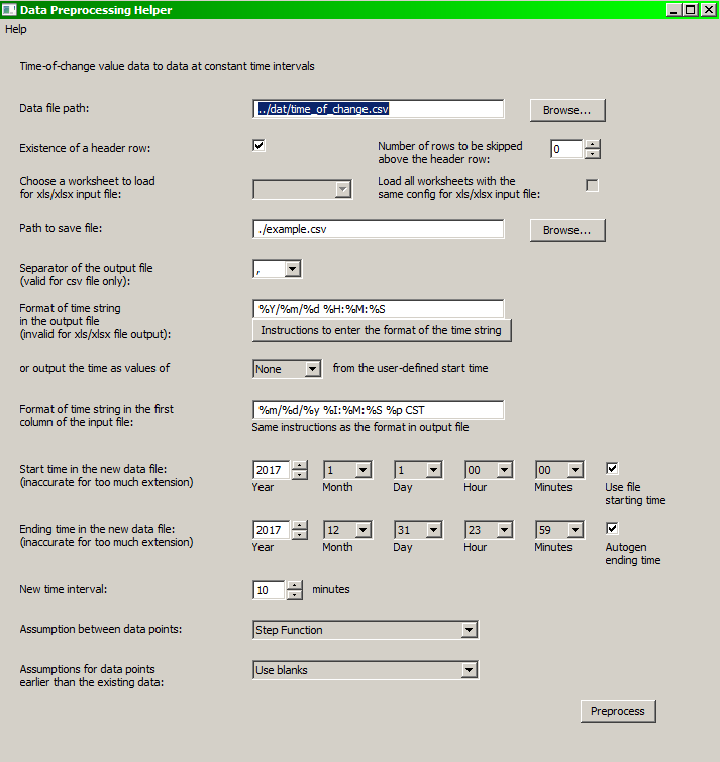
\includegraphics[width=0.6\textwidth]{ui.png}
\caption{Graphical user interface of the tool}
\label{fig:ui}
\end{figure}

To use the tool, use the first "Browse..." button on the right to choose the data file that you want to convert, and click the second "Browse..." button on the right to choose the directory where you want to save your file. Currently, it supports csv file (\href{https://en.wikipedia.org/wiki/Comma-separated_values}{Comma-separated Value File}), xls file (Microsoft Excel 1997-2003 File) and xlsx file (Microsoft Excel Open XML Format File). The locations of the two "Browse..." buttons are shown in Figure \ref{fig:ui_zoomed}.

\begin{figure}[H]
\centering
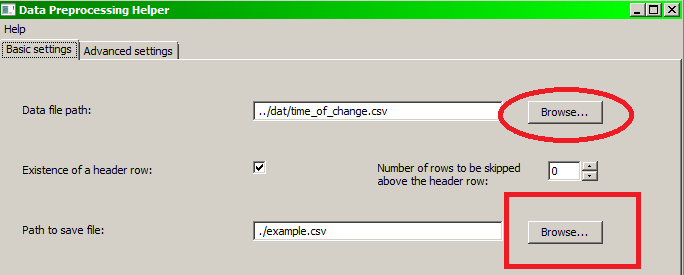
\includegraphics[width=0.6\textwidth]{ui_zoomed.png}
\caption{Location of the first "Browse..." button (in a circle), the second "Browse..." button (in a rectangle) and the text box for entering the format of the time string in the data file (in a pentagon)}
\label{fig:ui_zoomed}
\end{figure}

After that, you need to enter the format of the time string on the leftmost column of your data. The default setting is '\%m/\%d/\%y \%I:\%M:\%S \%p CST' supports a format which looks like

12/31/17 7:32:15 AM CST

. Other typical example of time string is shown in Table \ref{tb:sample_timestring}.

\begin{table}[H]
\caption{Sample format string for different types of time string in the data file}
\begin{tabular}{|p{6cm}|l|}
\hline
Format time string to be entered in the tool & Example time string being support \\ \hline
\%m/\%d/\%y \%I:\%M:\%S \%p CST & 12/31/17 7:32:15 AM CST  \\
 & 1/15/17 11:33:05 PM CST \\ \hline
\%Y/\%m/\%d \%H:\%M:\%S & 2017/12/31 13:00:30  \\
 & 1998/01/32 01:23:02 \\ \hline
 \%y-\%b-\%d \%I:\%M \%p & 99-Jan-01 12:01 AM \\
 & 00-Feb-31 01:08 PM \\ \hline
\end{tabular}
\label{tb:sample_timestring}
\end{table}

Details of their meaning can be found \href{https://docs.python.org/3.5/library/datetime.html\#strftime-and-strptime-behavior}{here}.

After that, all you need is to press the "Preprocess" button on the right hand corner, and you will have your file when the dialog box in Figure \ref{fig:complete} appears.

\begin{figure}[H]
\centering
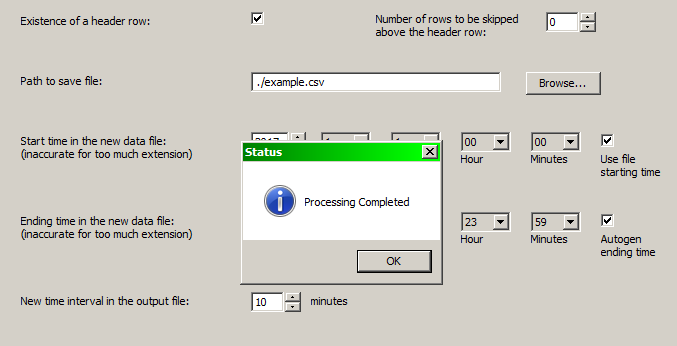
\includegraphics[width=0.6\textwidth]{complete.png}
\caption{Dialog box showing completion}
\label{fig:complete}
\end{figure}

And you can open the file at your selected location as Figure \ref{fig:step}

\begin{figure}[H]
\centering
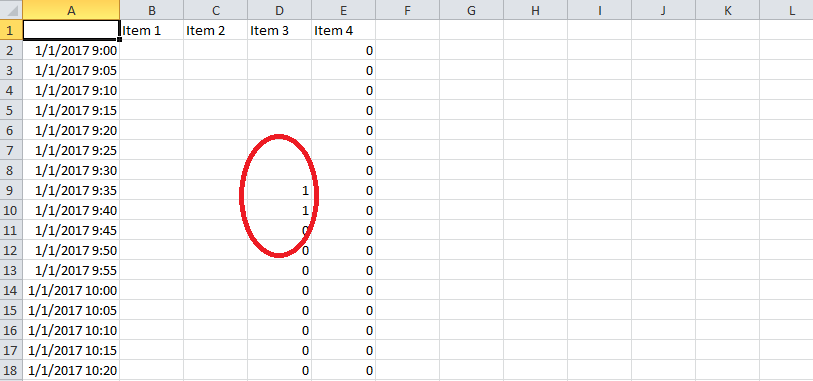
\includegraphics[width=0.4\textwidth]{step.png}
\caption{Pre-processed file}
\label{fig:step}
\end{figure}

There are other functions in the tool such as changing the time interval in the output file, using interpolation instead of step function, etc..
While they are available for you to explore in this version of tool, their documentation has not been completed.
Details of the functions will be discussed in documentation in future versions.

\subsection{Filling in invalid data points in a data file collected at fixed time interval}
\label{sec:tutorial_invalid}

This tutorial demonstrates how to use the tool to fill in invalid data points collected at fixed time interval.
To start the tutorial, we can consider the \emph{missing\_data.xls} file as shown in Figure \ref{fig:missing_data}.

\begin{figure}[H]
\centering
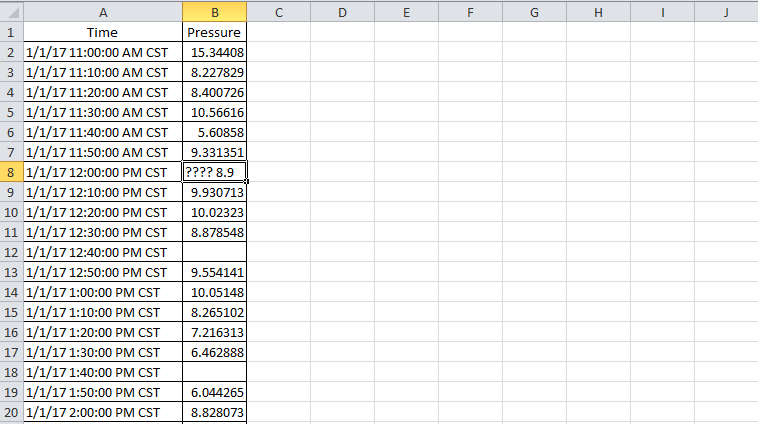
\includegraphics[width=0.6\textwidth]{missing_data.png}
\caption{Example data file with invalid and missing data points collected at 10-minute interval}
\label{fig:missing_data}
\end{figure}

Figure \ref{fig:missing_data} shows a file which data contains the following problems
\begin{itemize}
\item String characters within a data point at noon
\item Multiple data points without any values
\end{itemize}

To fix the file, we can conduct interpolation with the data adjacent to these problematic data points and fill them in with data from the interpolation.
To do so, we open the graphical use interface and choose the followings.
\begin{itemize}
\item Data file path: click "Browse..." to choose the file \emph{MissingData.xls}
\item Existence of a header row: checked
\item Number of rows to be skipped above the header row: 0
\item Choose a worksheet to load for xls/xlsx file: Sheet1
\item Load all worksheets with the same config for xls/xlsx input file: Unchecked
\item Path to save file: click "Browse..." and choose the directory and file name which you want to save the output file
\item Format of the time string in the output file: \%Y/\%m/\%d \%H:\%M:\%S (default)
\item output the time as values of: None
\item Format of time string in the first column of the input file: \%m/\%d/\%y \%I:\%M:\%S \%p CST
\item Start time in the new data file: Remain unchanged
\item Use file starting time: checked
\item Ending time in the new data file: Remain unchanged
\item Autogen ending time: checked
\item New time interval: 10 minutes (same as that of the file)
\item Assumption between data points: Continuous variable (inter- and extrapolation)
\item Assumptions for data points earlier than existing data: Use blanks
\end{itemize}

The output file should have the invalid and missing data points filled while other data points should remain unchanged as shown in Figure \ref{fig:missing_data_result}.

\begin{figure}[H]
\centering
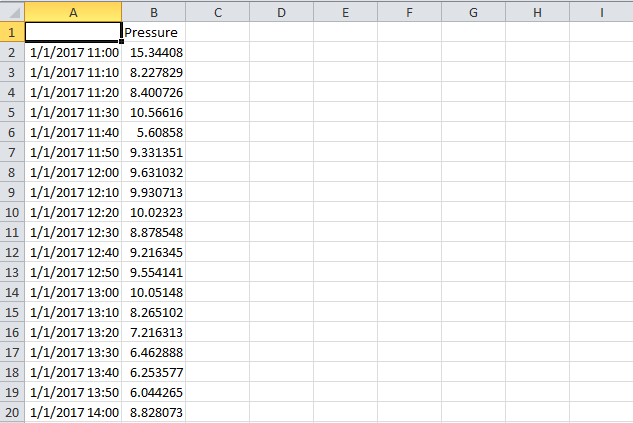
\includegraphics[width=0.6\textwidth]{missing_data_result.png}
\caption{Resultant data file after interpolation}
\label{fig:missing_data_result}
\end{figure}

\subsection{Using numerical values instead of string in the first time column}
Sometimes a user may want to use numerical values like hours or minutes instead of strings in the first column of time data.
This software also allows a user to convert the time column into numerical values as well.
Using the same example file in Section \ref{sec:tutorial_invalid}, a user simply need to change one option as follows:
\begin{itemize}
\item output the time as values of: minutes
\end{itemize}

and the preprocessing result will create a time column with numeric values of minutes from the start time of the file as shown in Figure \ref{fig:minute_data}.

\begin{figure}[H]
\centering
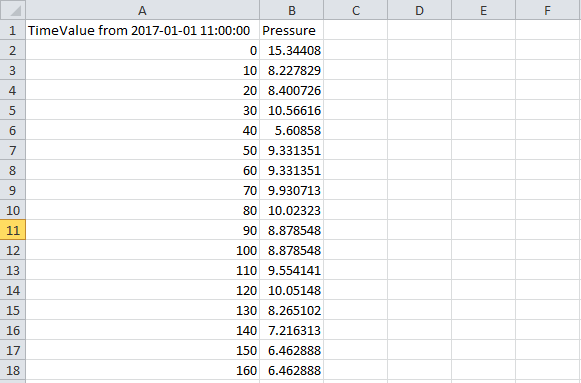
\includegraphics[width=0.6\textwidth]{missing_data_result_minute.png}
\caption{Resultant data file after interpolation with time column shown in minutes after the start time of the file}
\label{fig:minute_data}
\end{figure}

\section{Detailed input description}
This section gives details for each input in the graphical user interface in Figure \ref{fig:ui}.

\subsection{Data file path}
A user can enter the path to the file where the data should be preprocessed by the data preprocessing helper.
He or she can either enter the path manually in the box next to it, or use the "Browse" button to select the file requiring the preprocessing.

\subsection{Existence of a header row}
A user can specify if the data file contains a header row.
If the box is checked, the row in the data file will be considered as the header of the data table and will be output as the header in the output file.
If it is not checked, the first row of the file will be considered as the first row of the data file and the output file will be output with a default header row.

\subsection{Number of rows to be skipped above the header row}
Sometimes a data file may contain other information above the table of data.
If that's the case, specify the number of rows of redundant information in the data file in this box.
These rows will be ignored in the preprocessing.

\subsection{Choose a worksheet to load in xls/xlsx file}
If the data file to be processed is a xls/xlsx file, a user can choose the worksheet to be preprocessed in this drop down list.

\subsection{Load all worksheets with the same config for xls/xlsx file}
If all worksheets contain data that are formatted in the same manner (e.g. same format of time string in the first column, same number of rows above header, etc.), a user can preprocess the data in all worksheets simultaneously by checking this box.
Please notice that the output file must be an xls/xlsx file for the preprocessing to be successful.

\subsection{Path to save file}
A user can specify the directory and the name of the file to be saved.
They can either enter the path manually or use the "Browse" button to specify the location.

\subsection{Separator of the output file}
A user can choose the separator of the columns in the output file with two options: "," and ";".

\subsection{Format of time string in the output file}
\label{subsec:format_time_output}
A user can specify the format of the string in the output file here if the output file is in csv format.
The specification method can be found in paragraphs right below Figure \ref{fig:ui_zoomed}.
For xls/xlsx output files, the time data will be formatted following the Date/Time format in Microsoft Excel file.

If the user does not want to use any string or Microsoft Excel Date/Time format in the output file, they can specify the time column to be output as numerical time values since the start time of the output file.
This is done by specifying the option in the drop down list below the input field "Format of time string in the output file", and the choice of the output format includes "seconds", "minutes", "hours" and "days".

\subsection{Format of time string in the first column of output file}
A user should specify the format of the time column in the data file in this input field. The specification method is same as the one in Section \ref{subsec:format_time_output}.
Please notice that users can leave it to default values if the time column data in the original file is stored in Microsoft Date/Time format.

\subsection{Start time in the new data file}
A user can specify the start time in the new data file.
If the start time is earlier than the earliest time specified in the data file, a user can choose the assumption to predict the values of the data points before the earliest time in the input data as described in Section \ref{subsec:early_dat}.
Otherwise, the value at the start time will be calculated following the assumption of the relationship between data files as described in Section \ref{subsec:assume_bet_dat}.

\subsection{Use file start time}
If this checkbox is checked, the data preprocessing helper will use the time on the first row of the data as the start time in the output file.
The input in the input field "Start time in the new data file" will be ignored.

\subsection{Ending time in the new data file}
A user can specify the ending time in the output data file.
If the ending time is later than the last entry in the input data file, the assumption in Section \ref{subsec:assume_bet_dat} will be used to predict the values of the data at the end of the output file.

\subsection{New time interval}
A user can specify the time intervals between data points in the output file in minutes.
Please note that the input must be an integer.

\subsection{Assumption between data points}
\label{subsec:assume_bet_dat}
A user can choose the assumption of the values between the data points in the input file.
They can be either

\begin{itemize}
\item Step function
\item Continuous variable (inter- and extrapolation)
\end{itemize}

This helps to predict the values for data in the new output file which corresponding time has no record in the input data file.
Please note that the extrapolation and interpolation uses linear interpolation method.

\subsection{Assumptions for data points earlier than the existing data}
\label{subsec:early_dat}
A user assumes the values of data in the output data file which the corresponding time is earlier than the earliest time in the input data file. They can be either

\begin{itemize}
\item Use the minimum value in the trend
\item Use the first value in the trend
\end{itemize}

.
For the first option "Use the minimum value in the trend", the data preprocessing helper finds the minimum values of the data in each column in the input data file, and assumes that all data occur before the input file time period are maintained at these minimum values.
For the second option " Use the first value in the trend", the data preprocessing helper uses the first valid value in each column of the input file to predict the values of the data points earlier than the input file.

\section{Inquiries}

If you encounter bugs about the tool, please send an email to me at howard.at (at) gmail.com or post an issue at \href{https://github.com/howardcheung/data-preprocessing-helper/}{the GitHub repository}.

\section{License}

Please refer to the website at \href{https://github.com/howardcheung/data-preprocessing-helper/}{the GitHub repository} for the most up-to-date information about the licenses.

\section{Acknowledgement}

The developer(s) would like to acknowledge the followings for the inspiration and resources for the development of the software.

People (in alphabetical order of the family name):
\begin{itemize}
\item Dr. Diance Gao at Sun Yat-san University
\item Prof. Shengwei Wang at the Hong Kong Polytechnic University
\item Mr. KL William Wu at the Hong Kong Polytechnic University
\end{itemize}

Project (in alphabetical order of the project name):
\begin{itemize}
\item Energy Performance Assessment and Optimization on Buildings in PolyU Campus - Stage 1 and Whole Campus at the Hong Kong Polytechnic University
\end{itemize}

\end{document}